% -----------------------------------------------
% Template for SMC 2024
% Adapted from previous SMC paper templates
% -----------------------------------------------
\documentclass{article}
\usepackage{smc2024}
%%%%%%%%%%%%%%%%%%%%%%%% Some useful packages %%%%%%%%%%%%%%%%%%%%%%%%%%%%%%%
%%%%%%%%%%%%%%%%%%%%%%%% See related documentation %%%%%%%%%%%%%%%%%%%%%%%%%%
\usepackage[caption=false, font=footnotesize]{subfig}% Modern replacement for subfigure package
\usepackage{paralist}% extended list environments
\usepackage[figure,table]{hypcap}% hyperref companion

% The following command enables line numbers and it is meant for Review only
% it must be removed/commented out for Camera Ready version
%\pagewiselinenumbers


% Use this if english is the only language/alphabet used in the document
%\usepackage[english]{babel}
%--------------------------------------
% Japanese, Chinese, Korean
\usepackage[whole]{bxcjkjatype}
%\usepackage[japanese, main=english]{babel} % Does not work with plain pdfTex

%--------------------------------------
% Cyrillic
% The support is not perfect, diacritics are not working
%\usepackage[T2A,T1]{fontenc}
%\usepackage[russian, main=english]{babel}
%--------------------------------------
% Greek
%\usepackage[LGR,T2A,T1]{fontenc}
%\usepackage[greek, russian, main=english]{babel}
\usepackage{alphabeta}
%--------------------------------------
% HIGHLY EXPERIMENTAL, DO NOT USE AS IS.
% Arabic, Farsi, and Hebrew
\usepackage{arabtex}
\usepackage[LFE,LAE,LGR,T2A,T1]{fontenc}
%\usepackage[farsi, arabic, greek, russian, main=english]{babel}
\usepackage[greek, russian, main=english]{babel}
%--------------------------------------
% If more languages are needed please add the relevant packages


% Title.
% ------
\def\papertitle{A speaker agnostic approach to spatialisation in electroacoustic music}

% Authors
% Please note that submissions are NOT anonymous, therefore 
% authors' names have to be VISIBLE in your manuscript. 
% Authors are entered as an ordered list, each one can be linked to multiple affiliations using the correct index.
% Available tags for authors are: \firstname \middlename \lastname \generation \originalname \email \orcid
% Available tags for affiliations are: \unit \department \institution \streetaddress \city \state \postcode \country \type
% type can take as value: University, Company, Music, Independent, Other
%
% \author[]{\mbox{\firstname{}\middlename{}\lastname{}\originalname{}\generation{}\email{}\orcid{}}}
% mbox force an author not to be split over multiple lines
\author[1]{\mbox{\firstname{Stefano}\lastname{Catena}\email{stefano.catena23@gmail.com}\orcid{0000-0001-7650-4203}}}
\author[2]{\mbox{\firstname{Henrik}\lastname{Frisk}\email{henrik.frisk@kmh.se}\orcid{0000-0003-1958-8484}}}

%Affiliations
\affil[1]{\institution{De Montfort University}\department{MTI$^2$ - Music, Technology and Innovation - Institute for Sonic Creativity}\city{Leicester}\country{United Kingdom}d}
\affil[2]{\institution{Royal College of Music in Stockholm (KMH)}\city{Stockholm}\country{Sweden}\affiliationtype{Music}}

% Complete setup stage
\completesetup

% Title.
% ------
\title{\papertitle}
% ***************************************** the document starts here ***************
\begin{document}
	%
	\capstartfalse
	\maketitle
	\capstarttrue
	%
	
	\begin{abstract}
While spatial audio technologies have developed dramatically in the last twenty years, the compositional approaches to spatialisation in electroacoustic music are still fragmented. No coherent and shared language for spatialisation exists yet, and it is often challenging to reproduce an electroacoustic piece in different space from the one it was conceived in.    
In this paper we delve deeper into an approach about spatial audio and spatialisation techniques in the electroacoustic arts called 'speaker agnosticism'. By introducing Lilla Salen, a multichannel system of up to 49 speakers in a dome like configuration, and the authors' compositions, we describe a method of treating the concert hall as an instrument irrespective of the number of speakers it contains, or their arrangement. This paradigm shift encourages an 'organic' approach to music spatialisation, steering away from the traditional 'Euclidean' mindset. Finally, this project hints at the possibility of 'touring' pieces: by treating multichannel systems rather as instruments. Thanks to current audio technologies it is possible to 'transcribe' works between concert halls without the musical intention of the composer being lost.
	\end{abstract}
	%
	
	\section{Introduction}\label{sec:introduction}

It is almost impossible to divorce space from sound. Even a sound emanating from an anechoic chamber communicates a lack of space so remarkable that the lack of space itself becomes its identity. When listening to a piano in a concert hall, or when we hear a bird singing in the forest, whatever spatial information is in the sound - the reverberation of the concert hall or the density of the forest - is embedded and becomes an integral part of the perception of the sound. 
Yet, in musicology the theoretical and analytical representations of musical elements has for centuries often been reduced to quantitative parameters such as pitch (frequency) and rhythm (time). Still, from a perceptual point of view, the space of a sound is a parameter intimately tied to its cognitive meaning, to the degree that two sounds that share the same rhythm, pitch and timbre may be interpreted very differently by a listener if they are spatially different. 
Many of the technologies developed for working with spatial audio are biased towards a particular understanding of what spatial audio is. 
This is even more noticeable in electroacoustic music, where the spatial component of sound is one of its key elements\cite{Smalley1997}. 

        \section{Background}
	\label{sec:background}

Since the introduction of the loudspeaker, spatialisation and the spatiality of sound have taken an increasingly important role in the electroacoustic arts. Works such as \textit{Gesang der Junglinge} (1955-56) or \textit{Kontakte} (1958-60) from Karlheinz Stockhausen make use of the technology present in the 1950’s to create an immersive musical scene and to exploit spatiality for a musical goal. \textit{Gesang der Junglinge} uses five groups of spatially separated loudspeakers\cite{Decroupet1998}, while \textit{Kontakte} uses a four-channel speaker layout to project sound. Another notable example is Xenakis’ \textit{Concrète PH} (1958) and the Bruxelles Pavillion for which he contributed a sound installation, where over 400 loudspeakers were positioned inside the building in order to create spatial trajectories and movements\cite{Lombardo2005}. In parallel, the acousmatic French school developed instruments and tools for the diffusion of electroacoustic composition in music halls: Pierre Henry and Jaques Poullin introduced in 1951 the potentiometre d’espace to manage sound diffusion, but it is only in the 1970’s that Francois Bayle uses an ‘orchestra of loudspeakers’, the Acousmonium to ‘interpret’ sound spatialisation in a concert setting\cite{Solomon2007}. John Chowning’s experiment with computer music and Doppler effects are also a notable example of historical use of spatialisation: his piece \textit{Turenas} (1971), for instance, is a four-channel composition that actively includes spatial cues to ‘trick’ the listener into perceiving the direction of a simulated source\cite{Chowning1977}. Also in the 70’s was the first-order Ambisonics was conceived by Gerzon where a B-Format audio signal is used to represent the sound field instead of the speaker information, and later decode such signals for any arbitrary speaker layout\cite{Zotter2019}. Today this a very common technology for spatialisation, recommended by internet content providers such as Google or YouTube.\footnote{https://resonance-audio.github.io/resonance-audio/discover/concepts} First Order and Higher Order Ambisonics (FOA and HOA) are some of the most popular spatialisation technologies used currently\cite{Peters2011}, even though in the last years technologies like Dolby Atmos have caught up remarkably in the electroacoustic arts, too. 

There is no shortage of research on the technologies of spatialisation and even though the situation has improved slightly, Blesser and Salter's statement that "although there is a vast body of scholarly work both on the physical acoustics of enclosed spaces and on perceiving acoustic parameters, the literature is relatively silent on the subject of how people experience aural space" still has some validity. They continue: "We know much about measuring acoustic processes and sensory detection, but less about the phenomenology of aural space"\cite{Blesser2009}. Malham and Myatt comments that historically, the greatest problem with spatialised music has been the lack of, not only a comprehensive theory of spatialisation, but also of simple means to control it. Although much work has since been done, there are still no obvious standards\cite{Malham1995}. Ambisonics, a method for sound spatialisation, is grounded in a solid theory, but a comprehensive understanding of sound localization should include a phenomenological knowledge of the relation between sound and space \cite{Barrett2010, Malham1995, Travis2009}. 
Hence, if the early experiments beginning in the 50's lacked standardized control systems and theory, much of which has been settled in the last two decades, a broad and discursive aesthetic theory based on practical, artistic applications of sound diffusion is still lacking.
Nowadays, the affordability of computing power and loudspeaker setups has increased the interest for large multichannel reproduction systems: one of the most famous is the BEAST (Birmingham ElectroAcoustic Sound Theater) that has evolved from its original ‘main eight’ to over 100 speakers \cite{Wilson_Harrison_2010}. Another notable example is Lilla Salen at the Royal College of Music in Stockholm (KMH) or the Sonosfera in Pesaro with 45 custom built loudspeakers \footnote{sonosfera.eu}.

While the technological advancements in spatial audio technologies have been remarkable and permitted a larger pool of composers and artists to access complex spatialisation techniques, no coherent and shared musicological framework has been developed to describe their musical use\cite{Kendall2007}. However, several theories and ontologies of space have been proposed: one of the most prominent is Smalley’s ‘spatiomorphology’\cite{Smalley1997} and his investigation on musical spaces\cite{Smalley2007}. His concepts of ‘composed space’, defined as “the space composed on the fixed media”, and ‘listening space’, where the composition is played back into, are particularly relevant. In our investigation, only the concept of ‘composed space’ is taken into consideration: our range of action is limited to the space as created and ‘recorded’ by the composer, and all other approaches to spatialisation (e.g. live diffusion, multimedia installations etc) will not be taken into consideration.
In his ‘On Sonic Art’, Wishart proposes and investigates a series of spatial motions, their combinations in a sort of ‘spatial counterpoint’ and their perceptual relevance\cite{Wishart1996}; Kendall tries to describe and categorize the attributes of ‘spatial imagery’\cite{Kendall2010} and Catena attempts to establish an atomic unit for the description of spatialisation\cite{Catena2022}.
It is also important to clarify terminology while talking about spatialisation: many times terms like ‘spatial audio’ and ‘spatiality’ may be confusing or wrongly used. Holbrook describes the term ‘spatial audio’ as a “set of tools and methods for how to represent and control sound material through a process of spatialisation”\cite{Holbrook2019}. Consequently, we can define spatialisation as the conscious compositional act of moving or placing sounds inside or outside a given space with an intended musical aim. While this definition is similar to Holbrook’s, he omits to recognize that instrumental music can also employ spatialisation techniques to convey a musical meaning. The term ‘spatiality’, instead, is used to describe a set of physical spatial qualities of sound, e.g. its reverberation, perceived distance etc..

Another problem of spatialisation and spatial music in the electroacoustic arts is its reproducibility: once a piece is composed in a studio or in a particular venue, it has been historically complicated ‘moving’ it from one place to the other. With amplitude based spatialisation technologies the number of channels in the audio file represents the number of physical speakers they need to address: a piece written for a 9.1 setup could not be faithfully reproduced in an octophonic ring. 
By adopting the concept of speaker agnosticism we intend to address a compositional challenge as well as attempt to develop a preliminary terminology for the field of spatialisation studies, i.e. the way spatial properties in music can be understood and conceptualized, by mainly focusing on a set of attributes of perceptual importance.
The term 'agnostic' has been preivously used to describe the MPEG-H standard for audio encoding and object-based spatialisation\cite{quackenbush2021}, but no study exists that has gone into details of what speaker agnosticism entails artistically. By means of focusing on spatial perception rather than using a Euclidian\footnote{By 'Euclidian' we intend a spatialisation method that relies on a geometrical set of values to describe the instantaneous positions of sound objects in space. This concept will be described in more detail in section \ref{sec:organic }} approach to spatialisation we aim to suggest a theory of speaker agnostic composition practice. 
	\section{Speaker agnosticism}
	\label{sec:speaker_agnosticism}

The spatial musical aspect of a piece does not necessarily need to take into consideration the actual physical speaker layout in the room in which it is going to be played in. Ambisonics is a technology that is speaker agnostic at its core since it represents a sound field excitation as spherical harmonics\cite{Zotter2019}, rather than hard coding spatial information into the different channels. Regardless of the technology, which may vary in the future, the most fascinating aspect is how speaker agnosticism influences the process of composition. As is found by Schumacher: “it is generally difficult to recognize sound trajectories in space when there are no supporting visual stimuli”\cite{Schumacher2022}, which makes Euclidian approaches for sound spatialisation musically ineffective. Yet, a Euclidean approach to space is most commonly used as the basis for the spatialisation interface both for Ambisonics and many other spatialisation technologies. 

Speaker agnosticism is the notion that assumes that spatiomorphologies\cite{Smalley1997} are independent of reproduction and encoding technologies, inducing a 'relativist' spatial thinking\cite{Harrison2010}. For example, it is more important that a sounds moves, rather than defining a precise spatial trajectory that is difficult to locate and perceive, perhaps distorting the real compositional intent. This relates to the concrete perception of the morphology of its placements or movements, and it is only relevant in conjunction with consideration of the sound and the feeling that the sonic material may evoke. For example, a sound coming from behind or from the sides may be perceived as scary and unexpected (a howling wolf from behind the listener can be described as eerie), while a sound placed in the front may evoke a sense of anticipation, engagement or clarity. However, going even further with a speaker agnostic mindset, one could even disregard the traditional concept of front and back or left and right. If all directions are deemed equally significant, only the listener's subjective location becomes crucial, making the listener experience the primary focus of the creative process.  %%follow on this

        \subsection{Organic vs Euclidean}
	\label{sec:organic }

To describe the difference between Euclidean and organic thinking of spatialisation it is useful to start with a practical example. Let's imagine to stand in a forest and to think about what we could hear: an open space, the rustling of foliage, birds singing and flying, cracking branches, insects buzzing and the sound of flowing water of a nearby river. In an organic way of thinking spatialisation of such sound scene one could differentiate between three main categories of spatiomorphologies: 
\begin{itemize}
    \item \textit{Movements}: sound motions, be they continuous or discontinuous, where a clear, perceivable, and coherent change in location of the sonic material is heard. Sound trajectories are a common example of spatial movements: the sound of flapping wings of a flying bird, or a the buzzing of a passing wasp. A different example, in a more musical context, can be seen in Barry Truax’s ‘Shaman Ascending’\footnote{https://www.sfu.ca/~truax/shaman.html}: the whole piece is based on a rotatory movement of a vocal sound, until the rotation becomes so fast that it cannot be heard anymore. Being composed for an 8-channel system, the sound is moved intermittently between speakers, rather than blended between them to create a smooth transition. From a perceptual point of view, I regard these two approaches similar: both create the perception of a motion, be it continuous or discontinuous, and therefore falling in the same category.
    \item \textit{Placements}: absence of motion. Whenever a sound is statically located and its position easily perceivable, we would call this spatiomorphology a placement. For example, the identifiable high frequency sounds of birds songs where they can be heard in their immovable position.
    \item \textit{Occupancy}: a diffused positioning of sound. For example the immersiveness of wind passing through foliage creating the perception of sound coming from all around the listener and effectively occupying a portion of (or the whole) spatial scene.
\end{itemize}

When thinking about sound in a 'spatial' manner, these are the categories in which spatiomorphologies can be formed concretely. Their combination creates the complex spatial structure of a piece, and their function and relation to the sound material generates the musical discourse. Moreover, it is not always important to think precisely \textit{how} these spatiomorphologies behave: for example, it is musically more relevant that a sound moves, rather than it moving from left to right (or viceversa); or that this sounds is placed in a specific location, rather than on its opposite side (even if this may not always be the case). However, in an organic thinking of spatialisation, it is the movement, the placement or the occupancy of sound to be spatially meaningful, and how the combination of spatio and spectromorphologies results in the creation of the musical structure. 

Conversely, a Euclidian approach to space considers spatiomorphologies a sound source described only by a set of geometrical coordinates, rather than looking at their spatial qualities. For example, in the iconic John Chowning's piece \textit{Turenas}, the composer creates spatial illusion of moving sources, along with Doppler effect, azimuth and distance manipulation \cite{Chowning2011}. Through his system, Chowning was able to design complex trajectories of sounds in space,  following Lissajous figures (as shown in Figure \ref{fig:turenas}) in a very precise geometric space. However, this approach was used in a quadraphonic setup, known for being an unreliable reproduction system for sound localisation and, more importantly, it would be impossible to accurately recognize and track the Lissajous figures, making them musically ineffective. 
        \begin{figure}[t]
		\centering
		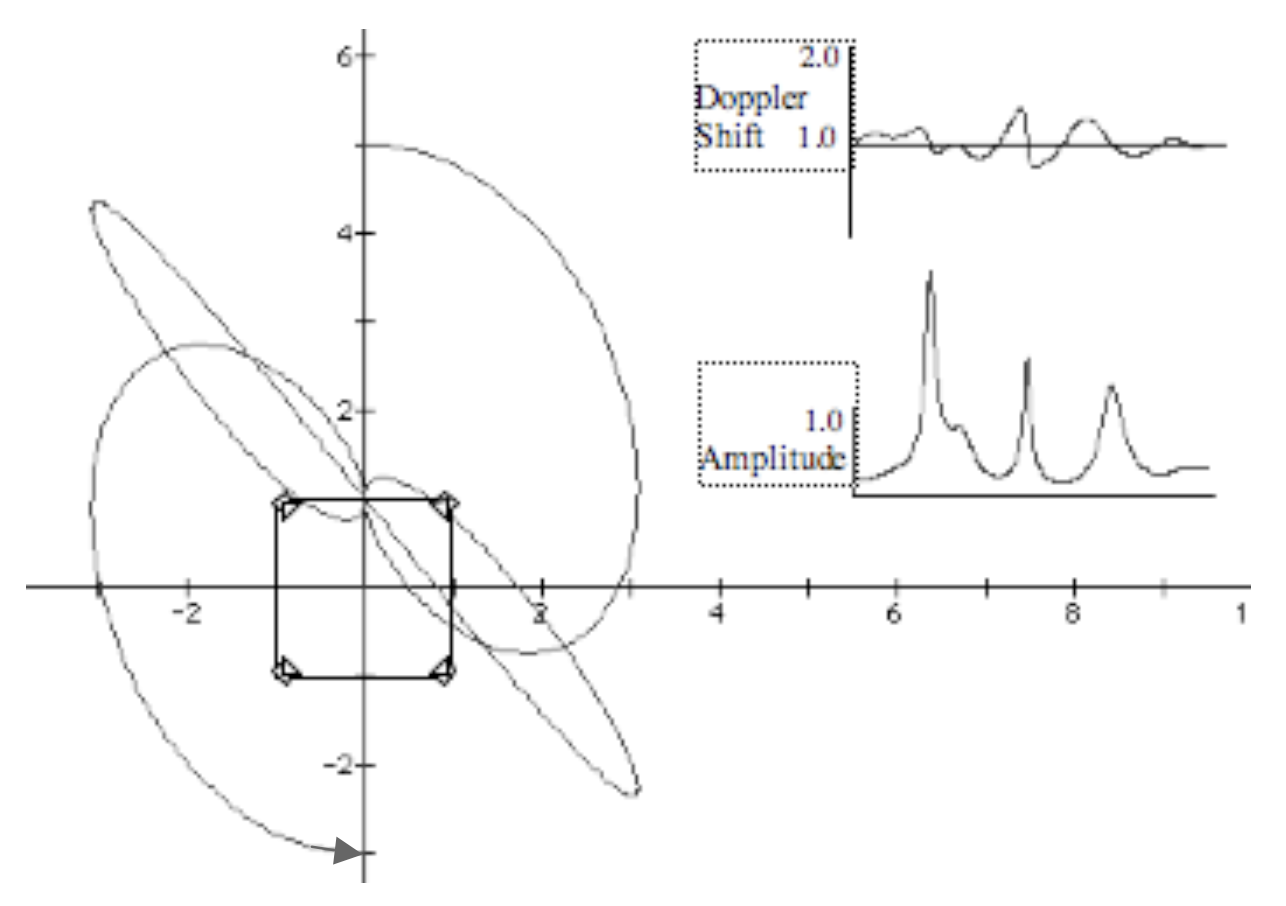
\includegraphics[width=1\columnwidth]{SMC_2024_Paper/Turenas.png}
		\caption{One of the Lissajous figure in \textit{Turenas}, with Doppler effect and Amplitude values\cite{Chowning2011}\label{fig:turenas}}
	\end{figure}  

These two methods for the compositional thinking of spatial music can be interpreted in terms of 'relativist' and 'absolutist'. The organic approach can be described as more 'relativist', where macro categories of spatiomorphologies are used to musically exploit their perceived spatial shapes and characters; the traditional Euclidian approach can be view as 'absolutist', where the spatial placements and movements follow a precise and 'objective' set of numeral descriptors, creating complex spatial structures. Our intention is to return to the subjective - i.e. organic - listening experience as the key source of knowledge for sound spatialisation in electroacoustic composition. This also includes the rejection of the power of the concert hall and technologically advanced multi speaker environments as an idealized place for virtual sound worlds, and instead make the act of composition the main spatial listening exercise. In this re-framed performance environment various forms of listening hold a central aspect of the spatiality of the music. Our concept of speaker agnosticism tries to shift the focus from the technology to the technique and to the listening experience.
However, not all organic or Euclidian approaches to spatialisation are necessarily speaker agnostic: these two ways of thinking the space relate only to how the composer approaches and creates the 'composed space'. In fact, speaker agnosticism relies on a suitable technology that permits a 'translation' between different multichannel systems, such as Ambisonics or Dolby Atmos. 

        \subsection{From technique to technology }
	\label{sec:technique}
 
 Most of the technology (both hardware and software) for spatialisation today follow a Euclidian approach to space. Whether it be Ambisonics, DBAP (Distance Based Amplitude Panner), VBAP (Vector Based Amplitude Panning), Dolby Atmos or others, one would have to specify geometrical coordinates for the positioning of the sound sources in space. This affects the way in which a composer places and moves sound in the piece. Moreover, due to this technological factor, it is inevitable to deal with some form of geometrical aspects during the spatisalisation act. One cannot avoid to specify azimuth angles or cartesian coordinates in their compositional workflow. However, if one were to establish and to think of general directions instead of geometrical coordinates, a different perspective for spatialisation arises. The perspective of a continuous space, rather than a discrete one, where the compositional process follows meaningful perceptual properties. This compositional process, in fact, would help and contribute to a speaker agnostic approach to spatialisation, since no technical information is required. By disregarding the intention of excessively localised trajectories and sound placements, it is possible to think of an idealised empty space to fill, rather than an actual physical multichannel system with speakers to address. Furthermore, by detaching the technological aspects from the work (i.e. thinking agnostically), the importance of the musical act is given back to the spatiomorphologies - and consequently to the listening experience. By using an algorithmic approach, for example, it would be easy to displace sound into perceptually relevant 'macro-directions': a relevant example is described in section \ref{subsec:approach}.
 
 \section{Compositional practice}
	\subsection{Travelling without moving}
        \label{sec:twm}

        \textit{Travelling without moving} is an acousmatic composition written at the KMH in Stockholm in 2023, specifically in the multichannel half dome present in Lilla Salen, that strongly incorporates the 'composed space' as one of its most important features. As the title suggests, the piece revolves around the concept of motion, movement or their absence: most of the sonic material can be heard while traversing the performance space, creating complex spatial textures and perspectives. However, in several key moments, the strategic static placement of the material will clash, contrast or complement the rest of the spatial scene. Moreover, another key component of the piece is the relationship between timbre and space: 'how the sound behaves' and 'how the sound moves' are the two intertwined ideas that are investigated musically. All the employed timbres come from the Buchla modular system (Figure \ref{fig:buchla}) present in the electroacoustic facilities of KMH. (insert image). Modulated oscillators (Dual Oscillator 258 and Quad Function Generator 281e) and noise generators (Source of Uncertainty 266) in conjunction with the Buchla's 'Spectral Processor 296e' were utilized to produce and shape the timbral material of the composition.   

        \begin{figure}[h]
		\centering
		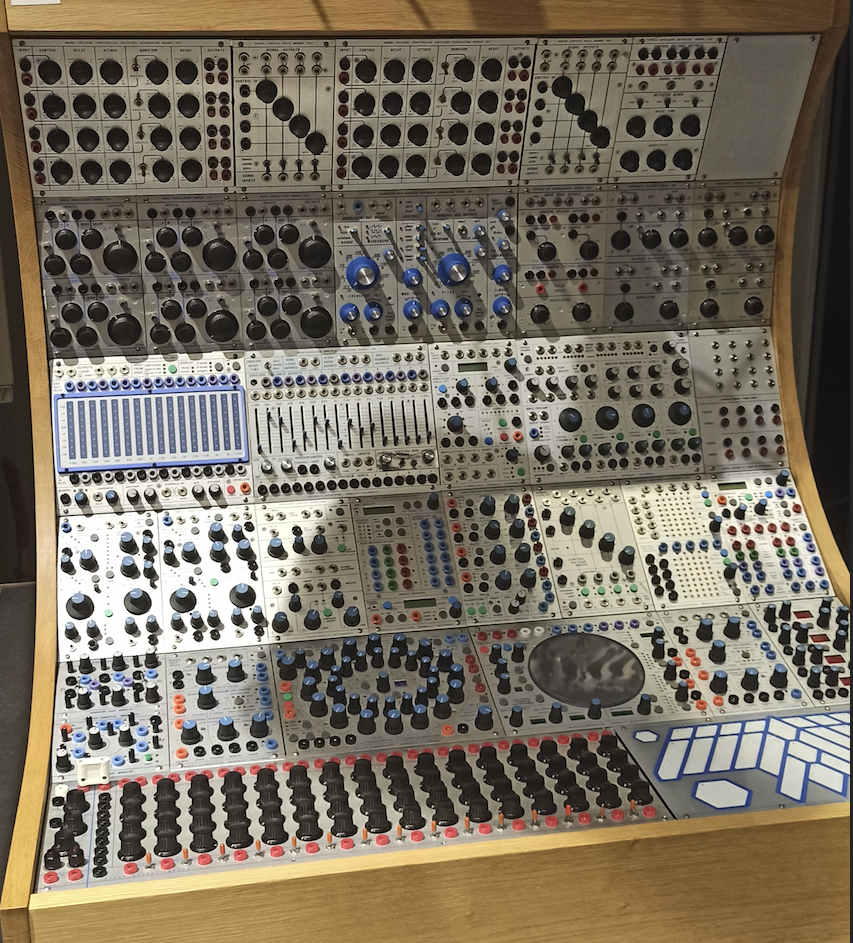
\includegraphics[width=1\columnwidth]{SMC_2024_Paper/buchla.png}
		\caption{The Buchla system present at the Royal College of Music facilities\label{fig:buchla}}
	\end{figure} 
        
        Algorithmic manipulation of the sonic matter and tape techniques were employed to further modify and recombine the recorded timbres as needed. The spectromorphologies that resulted from the sound generation and its consequent transformation have deeply influenced the compositional choices regarding spatialisation: the sonic material and its deployment in space are strongly linked and not independent from one another. For example, pitch and amplitude changes are most likely linked with a moving source that follows along the spectromorphological changes, while sounds that are strongly connected to natural environments (e.g. rain) would occupy large portions of the spatial scene, enveloping the listeners.
        The composition is structured in three main sections that follow one another in sequence:
        \begin{itemize}
            \item \textit{Departure}: the first section consists mostly of rotary timbres, similar to how a helicopter whirring would sound. These sound sources are split into several bands, where each portion of the spectrum is moved around the listener to create an enveloping texture of moving objects. This first section represents a departure from the real-world and into another sonic and spatial environment, where the mind is free to travel where it wants.
            \item \textit{Travelling}: when the first section ends, relaxing sounds of falling rain fade in and fully occupy the scene, just like waking from a dream after sleeping too much on a green grass field. From this soundscape various wandering objects emerge, collide and, through a process of accumulation and layering, create a complex texture of moving sounds from and to all directions, similar to a storm. After this storming climax, a slow and gradual decrescendo is present, leading to the next section. Both the climax and the decrescendo involve the transformation of all musical parameters: timbre, space, dynamic and pitch. 
            \item \textit{Landing}: the last section calls back to the relaxing sound of falling rain, but with the addition of several statically positioned sounds: insects and birds chirping are added to the soundscape, finally waking up the listener. Moving textures recall the travel and its climax, but they fade away like a forgotten dream. Eventually, within the synthesized sound of rain, a paradoxical 'immobile' sound of footsteps is heard, gradually dying out and closing the piece. 
        \end{itemize}
        
        Ideally, this piece should be played in venues that can accommodate multichannel reproduction in an hesa/octophonic setup at minimum; however, the piece is not strictly tied to a particular space or speaker. Thanks to Ambisonics technology, it is possible to decode the piece in any speaker layout present at any time, making the piece, by definition, speaker agnostic.
        The composition can be heard online in a binaural rendition.\footnote{https://soundcloud.com/stefanocatena/travelling-without-moving-binaural-version}
	
	\subsubsection{Approach to spatialisation in Lilla Salen}
	\label{subsec:approach}

        As mentioned, \textit{Travelling without moving} has been composed at the Royal College of Music in Stockholm, more precisely with the multichannel half dome system in the concert hall called Lilla Salen.

        \begin{figure}[h]
		\centering
		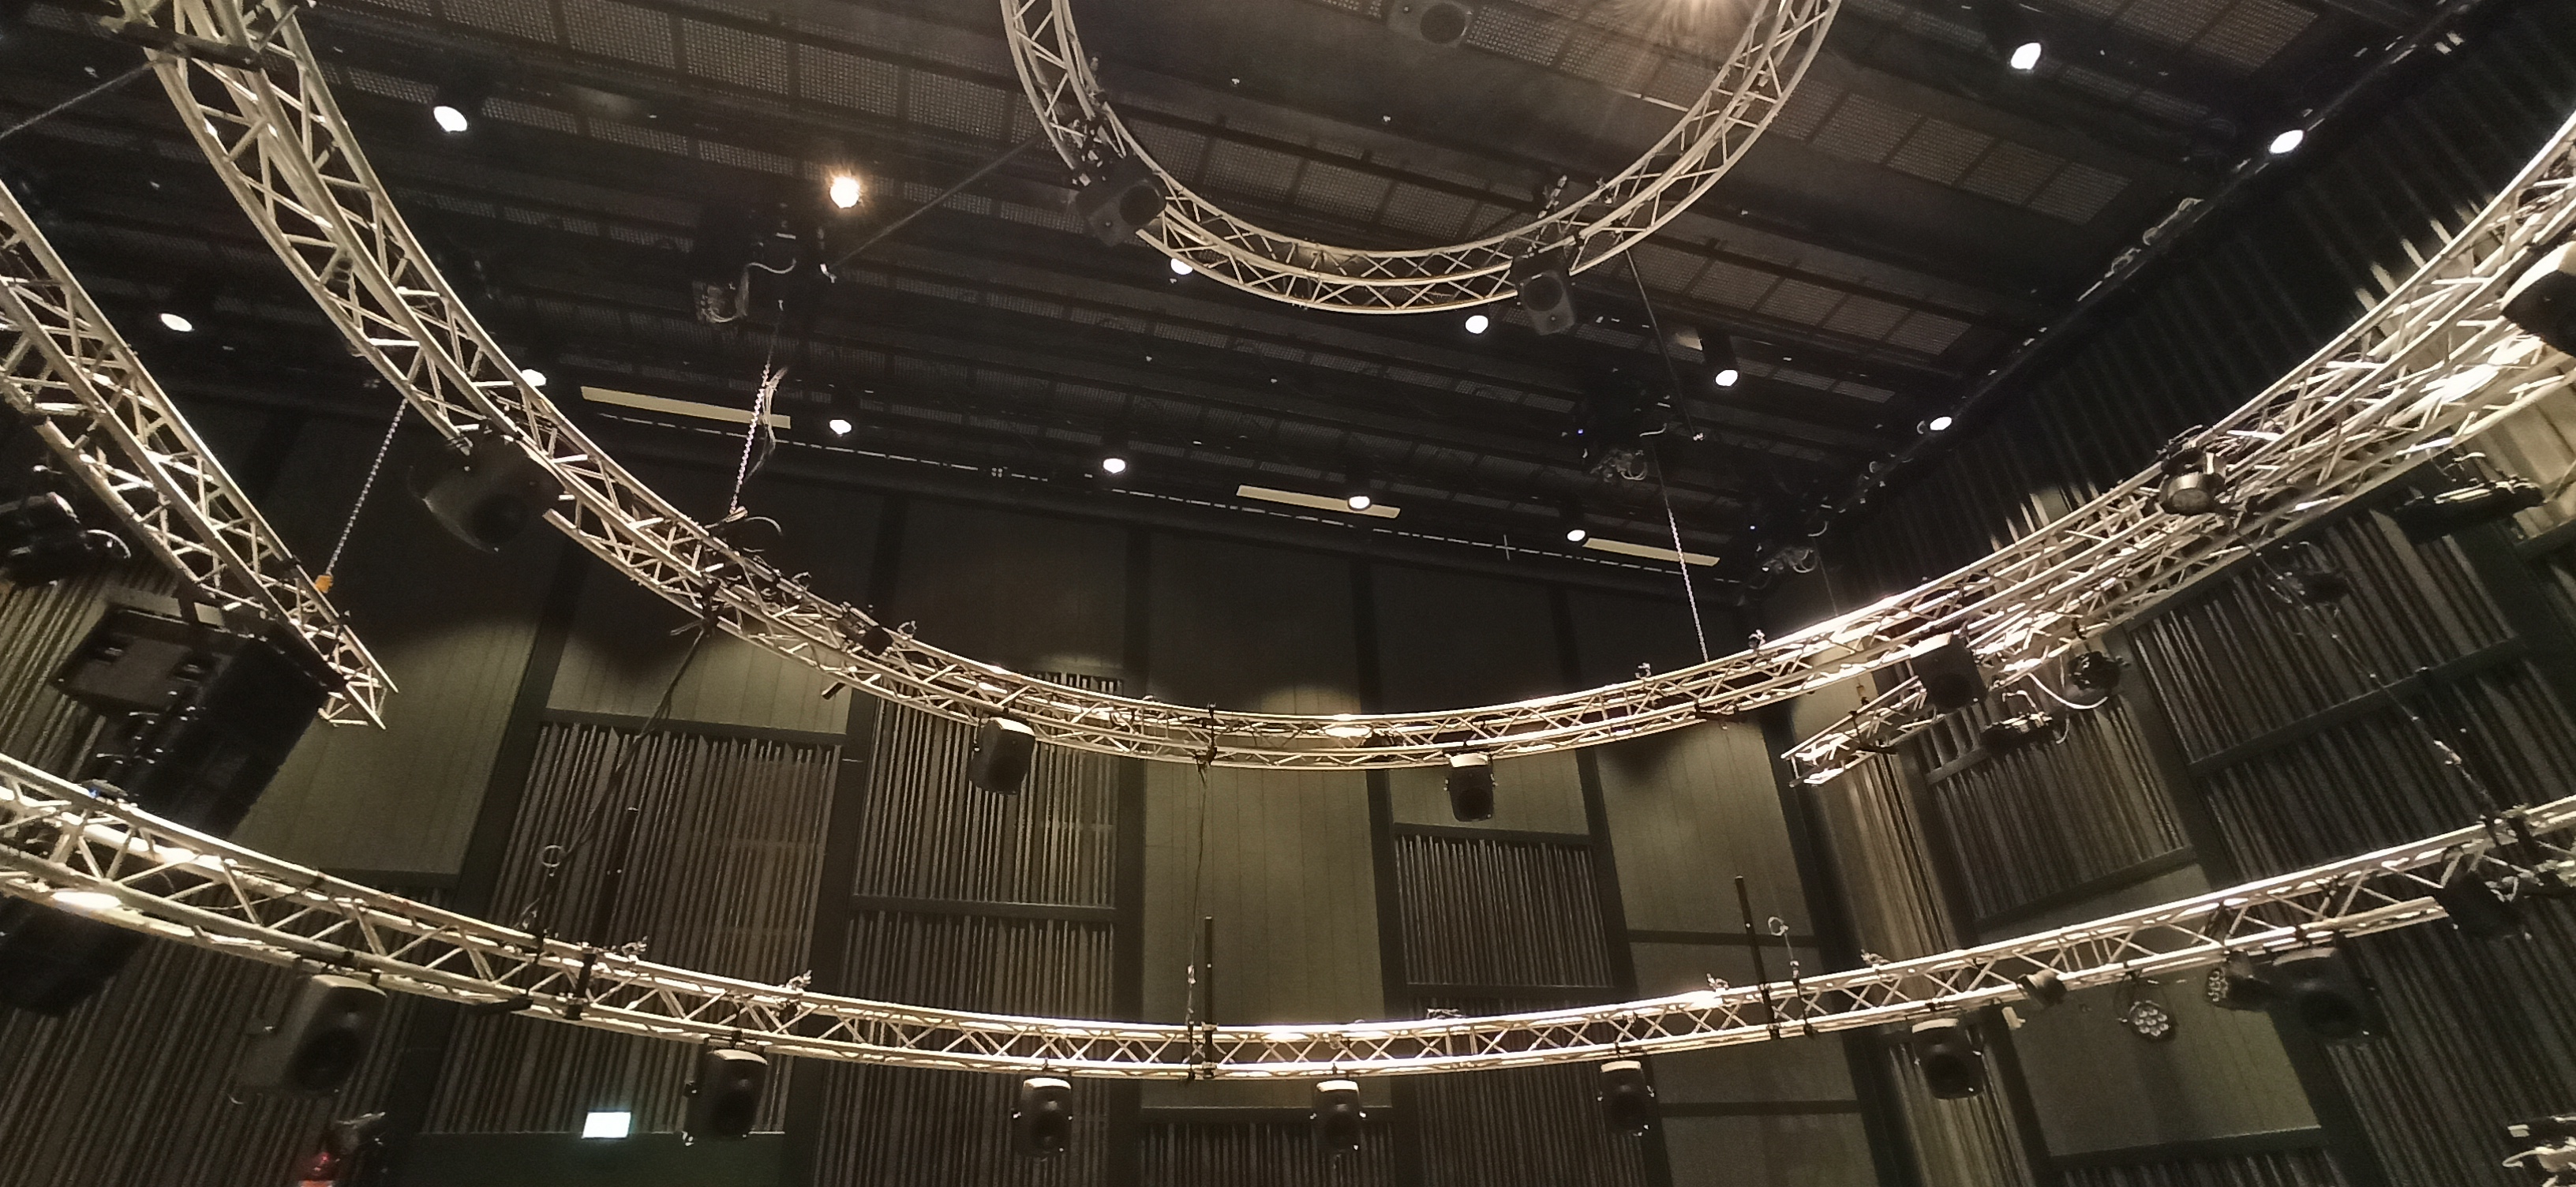
\includegraphics[width=1\columnwidth]{SMC_2024_Paper/lillaSalen.jpg}
		\caption{Lilla Salen\label{fig:lilla}}
	\end{figure}  
        
        Lilla Salen at KMH (shown in Figure \ref{fig:lilla}) is configured for both research and experimental performance. A flexible system of up to 49 loudspeakers in a dome like configuration affords a platform for a wide variety of projects including sound spatialisation either in the acousmatic tradition or with acoustic and electronic instruments together. The system creates an immersive sound environment while providing precise sonic imaging for studies in spatialisation and cognition. Merely describing a space like Lilla Salen reveals the focus on the technological aspect of the room and for the composer working in this space it tends to put the focus on how to handle the speaker layout and the structurality of the technology in the hall. How the various inputs and outputs are configured tends to allow, or disallow, particular practices. The vision that a spatialisation technique such as Ambisonics fosters that spatial music can be agnostic towards speaker layouts and performance spaces is challenged by this. To instead treat the hall as an instrument, a specificity rather than a general space for listening and creation, is an alternative approach. Then any new rendering of such a piece for a different hall is an interpretation much more than an exact replica. In fact, the spatial approach and thinking while composing the piece does not take into consideration the technical aspects of the hall, but rather exploits and treats the space for what it is: a half dome.\\
     \begin{figure}[h]
	\centering
	\hspace*{-1.25cm}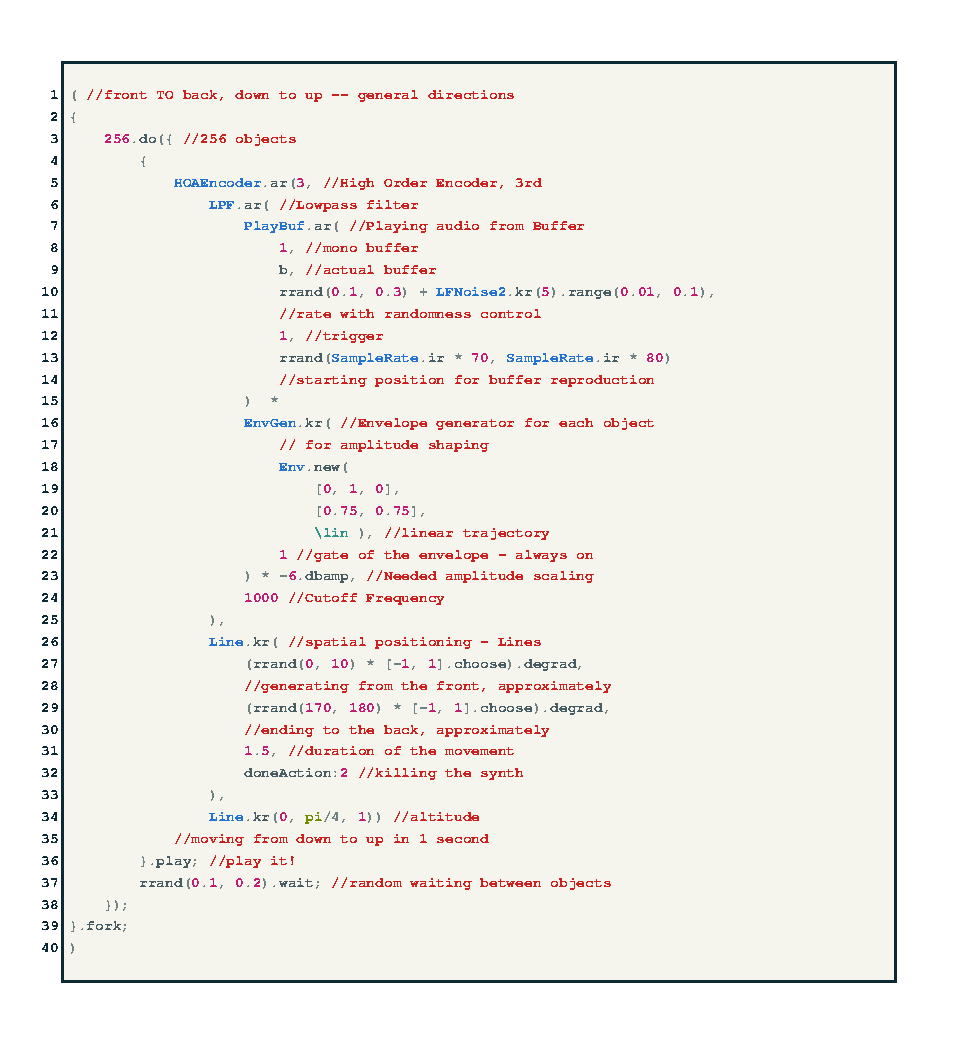
\includegraphics[scale = 1, width = 10cm]{SMC_2024_Paper/code.pdf}
	\caption{Example of a routine that generates complex spatial textures from single moving objects using Higher Order Ambisonics in Supercollider\label{code}}
\end{figure}
        A speaker agnostic thinking of the space encourages an algorithmic approach to spatialisation. With the term 'algorithmic' we intend "the application of rigid, well-defined algorithms to the process of composing music"\cite{Jacob1996}. By generating several takes of spatialised material, it is crucial to 'compose' the desired texture after a critical listening. This algorithmic method allows to not think of space mathematically - i.e. Euclidian thinking - but rather to listen to how the space is generated, how the sounds moves, how it occupies portions of the space, the interconnections created between spectro and spatiomorphologies. Ambisonics is the ideal technology for this approach, as it is able to intertwine sound and space at their inception and decode the spatial information for any kind of speaker layout. Moreover, its flexibility and ease of use has made it the optimal companion of programming langugages such as Supercollider\footnote{https://supercollider.github.io} or Max/MSP from Cycling 74\footnote{https://cycling74.com}. In this case, Supercollider was the preferred language from the author, since it has historically handled multichannel signals reliably.

        This method has been used all throughout \textit{Travelling without moving}. From 2:15 to 5:20, for instance, all the spatialisation adopts exclusively this approach, creating the ever-moving spatial fabric with several recordings algorithmically generated, carefully chosen, organised and timbrically modified. \\
        From the example shown in Figure \ref{code} it is possible to see how there is no Ambisonics decoder present. This is a very specific compositional choice that leads to an organic process in creating the space. To include a decoder would mean to translate a speaker agnostic signal (the B-format) to a physical speaker layout. By doing this one could be biased to 'compose for the space', rather than 'compose the space': in fact, it could be argued that with this approach we are composing (for) the Ambisonics B-format. In this example, while we inevitably specify geometrical coordinates in the code, it is also noticeable the 'relativism' in creating the spatiomorphologies. The randomness present at lines 27 and 29 from Figure \ref{code} represent the intention of not producing pre-determined specific trajectories, but rather that pseudo-random motions moving from and to macro-directions will form and coalesce into a spatial texture of musical meaning. It is also important to notice that Higher Order Ambisonics has been used: in line 5 of Figure \ref{code} the HOA encoder and its order is specificed. By increasing the Ambisonics order more spherical harmonics are introduced, which increseas spatial accuracy, directional resolution and enlarges the sweet-spot\cite{Zotter2019}. However, for the Higher Order Ambisonics B-format a large number of channels is required, which equals to $(n+1)^2$ where $n$ is the Ambisonics Order: for instance, a third order B-Format uncompressed .wav file is made up of 16 channels.

        Eventually, the physical attributes of the space will have to be determined: however, this last process can be considered outside of the compositional system, as it is not involved in any way in the writing of the musical piece, but is rather only an infrastructure that aids the listening experience and audio monitoring. In fact, thanks to IEM\footnote{https://plugins.iem.at} audio plugins for Ambisonics workflow, one could quickly switch between multichannel or binaural listening, based on contingency or preference. In the case of \textit{Travelling without moving}, the audio monitoring has been primarily provided by the system in Lilla Salen, but in many cases the binaural renderer has helped the process as an immediate and accessible reference. The Ambisonics decoder used for the Lilla Salen monitoring system can be found in the author's Github repository:\footnote{https://github.com/friskgit/kmh{\_}ls} in this case the IEM AllRad Decoder has been used.\footnote{https://plugins.iem.at/docs/allradecoder/}

    \subsection{For Bill, Rising}
    \textit{For Bill, Rising} is in a sense inspired by James Tenney's \textit{For Ann, Rising} although it does not have much sonic references to it. The basic idea behind this composition is to use a simple synthesis model, in this case a snare drum, and create timbral variations through combining repetitions of the original sound and spatialising them differently. The tonality and the rhythm is derived from the 7-limit, 11-note scale shown in Figure \ref{fig:score}. In the piece rhythms are treated as slowed down intervals and vice versa. The form is structured around a rather simple presentation of the scale and the harmonic and melodic material emanates from it. Originally, the piece is constructed using a variety of different techniques for spatialisation, departing from the notion that each sound has its own spatial properties already at the time of its generation. Hence, the piece is not synthesized and then spatialised, but space is composed into the sound. The technique used for the spatialisation is vector based, but the final representation is rendered in ambisonics. The composition can be heard online in a binaural rendition.\footnote{https://soundcloud.com/mail-97/for-bill-rising}

    \begin{figure}
        \centering
    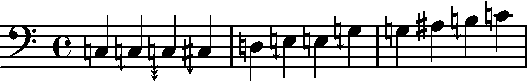
\includegraphics[width=\linewidth]{SMC_2024_Paper/micro.pdf}
        \caption{Basic scale for the melodic, harmonic, and spatial structure of \textit{For Bill, Rising}}
        \label{fig:score}
    \end{figure}
    
     Basically, the piece is a step wise motion from the root of the scale and upwards until the octave is reached at which case the piece has reached its end (See Figure \ref{fig:score}). The basic spatial direction, i.e. the centre of all spatial movement, for each of the twelve sections of the piece corresponds to the relative angle of each of the notes in the scale compared to the root. For example, the distance between the root and the first note in the scale is the distance betweeen $\frac{1}{1}$ and $\frac{81}{80}$ (roughly 21.5 cents) which is translated to the angle $6.45^{\circ} = 21.5/1200*360^{\circ}$. 
     In this manner all angles used for spatialisation in the piece are related to the intervals in the scale. In this sense the spatialisation of the piece is dervied from a Euclidean way of thinking. 
     At the same time, however, the spatiomorphology of the piece follows an organic thinking about spatialisation since all \textit{movements} are linked to the \textit{placements} and \textit{occupancies} in the piece.
     Even though the musical and spatial parameters are mathematically generated the perceptual and organic thinking can be observed here. 
     The focus on the space is composed \textit{through} the material, rather than the material being composed \textit{into} the space.
     \textit{For Bill, Rising} is to a high degree composed algorithmically in a similar fashion to \textit{Travelling without moving}, as described above.  
     It is an attempt to try to break with the common way of dividing the practice of composition into several interrelated stages and instead approach the synthesis of the material as an integrated practice.
     In this case it means that the parameters and the data for each musical gesture are used and allowed to influence several musical aspects--e.g. timbre, space, rhythm, harmony, and others--in the same process. 
     This integrated method of composition further emphasizes the organic modality of spatialisation, allowing space to evolve from within the sound, rather than something that is applied on top of the sound. 
     The timbre as well as the spatialisation of the sound are then functions of a mode of composition that departs from algorithmic thinking used to explore the musical material. 
     This participates in integrating spatialisation as a musical parameter along with the others, rather than an aspect that is added at the end. 
     In some sections of the piece spatialisation is used as a synthesis method, further blurring the lines commonly dividing the traditional compositional practice's sub tasks: synthesis, composition, mixing, spatialisation, etc.
     Just as for \textit{Travelling without moving}, in \textit{For Bill, Rising} this algorithmic process has been achieved using SuperCollider.
     Although the piece was originally composed for the Lilla Salen hall at KMH, it has been rendered speaker agnostic through Ambisonics. 
     This has been achieved by re-recording it as a B-format Ambisonics. 
     The original piece was rendered using VBAP to a file with 29 channels, one for each speaker in the Lilla Salen Dome. 
     This file was transformed to a B-format signal by feeding each signal through a separate encoder panned to the appropriate position of the speaker in question.
     The difference between the original version using vector based techniques for spatialisation and the Ambisonics version is noticeable when the two versions are compared in Lilla Salen. 
     Some of the precision of the VBAP panning of single sound sources is blurred by rendering the piece in Ambisonics, as may perhaps be expected given the nature of both the process of encoding and the Ambisonics technology.
     However, the quality of the spatial impression of the more swirling sounds in the piece, as well as the distant sounds are generally improved in the Ambisonics version.
     The piece has been performed in a few other locations (Helsinki, Finland and Stanford, California, US) and in these cases the difference between the original version for Lilla Salen and the Ambisonics version is not noticeable.
     This process integrates well with the idea of speaker agnosticism.
 
	\section{Conclusions and further works}

    In this paper the concept of speaker agnosticism has been contextualised in the field of electroacoustic artistic practice, and the differences between two contrasting ways of thinking about compositional space, organic and Euclidian, has been described. 
    This work focuses on listening as the main drive for the spatial compositional process, independent of the technological and technical aspects of spatialisation, but also on the algorithmic possibilities as derived from this process. 
    However, speaker agnosticism and the organic modality of space can be a new way to approach the development of technologies for spatialisation, as well as helping the 'translation' of electroacoustic pieces between different multichannel speaker systems. 
    Following the results of this work,  we see that it would be possible to institute a 'network' of coordinated concert halls that share technical information that provides support to composers and that promotes aesthetic discussion and development in this field. 
    Composers could create 'touring' pieces, where an electroacoustic work composed in Stockholm, for example, could be performed in Leicester maintaining the same spatial musical intent. 
    The introduced pieces, \textit{Travelling without moving} and \textit{For Bill, Rising}, follow this idea: their spatial relevant musical information is kept by using a suitable current technology - Ambisonics, in our case - and by approaching spatialisation from an organic and speaker agnostic perspective.

   

 
	\begin{acknowledgments}
    This project has been possible thanks to the Arts and Humanities Research Council (AHRC) and the Midlands4Cities (M4C) doctoral consortium that have funded the author's residency at the Royal College of Music of Stockholm in June-July 2023.
	\end{acknowledgments} 
	
	%%%%%%%%%%%%%%%%%%%%%%%%%%%%%%%%%%%%%%%%%%%%%%%%%%%%%%%%%%%%%%%%%%%%%%%%%%%%%
	%bibliography here
	\bibliography{smc2024bib}
	
\end{document}
